%%%%%%%%%%%%%%%%%%%%%%%%%%%%%%%%%%%%%%%%%
% Short Sectioned Assignment
% LaTeX Template
% Version 1.0 (5/5/12)
%
% This template has been downloaded from:
% http://www.LaTeXTemplates.com
%
% Original author:
% Frits Wenneker (http://www.howtotex.com)
%
% License:
% CC BY-NC-SA 3.0 (http://creativecommons.org/licenses/by-nc-sa/3.0/)
%
%%%%%%%%%%%%%%%%%%%%%%%%%%%%%%%%%%%%%%%%%

%----------------------------------------------------------------------------------------
%	PACKAGES AND OTHER DOCUMENT CONFIGURATIONS
%----------------------------------------------------------------------------------------

\documentclass[paper=a4, fontsize=11pt]{scrartcl} % A4 paper and 11pt font size

\usepackage{float}
\usepackage[T1]{fontenc} % Use 8-bit encoding that has 256 glyphs
\usepackage{fourier} % Use the Adobe Utopia font for the document - comment this line to return to the LaTeX default
\usepackage[english]{babel} % English language/hyphenation
\usepackage{amsmath,amsfonts,amsthm} % Math packages

\usepackage{graphicx}

\usepackage{sectsty} % Allows customizing section commands
\allsectionsfont{\centering \normalfont\scshape} % Make all sections centered, the default font and small caps

\usepackage{fancyhdr} % Custom headers and footers
\pagestyle{fancyplain} % Makes all pages in the document conform to the custom headers and footers
\fancyhead{} % No page header - if you want one, create it in the same way as the footers below
\fancyfoot[L]{} % Empty left footer
\fancyfoot[C]{} % Empty center footer
\fancyfoot[R]{\thepage} % Page numbering for right footer
\renewcommand{\headrulewidth}{0pt} % Remove header underlines
\renewcommand{\footrulewidth}{0pt} % Remove footer underlines
\setlength{\headheight}{13.6pt} % Customize the height of the header

\numberwithin{equation}{section} % Number equations within sections (i.e. 1.1, 1.2, 2.1, 2.2 instead of 1, 2, 3, 4)
\numberwithin{figure}{section} % Number figures within sections (i.e. 1.1, 1.2, 2.1, 2.2 instead of 1, 2, 3, 4)
\numberwithin{table}{section} % Number tables within sections (i.e. 1.1, 1.2, 2.1, 2.2 instead of 1, 2, 3, 4)

\setlength\parindent{0pt} % Removes all indentation from paragraphs - comment this line for an assignment with lots of text

%----------------------------------------------------------------------------------------
%	TITLE SECTION
%----------------------------------------------------------------------------------------

\newcommand{\horrule}[1]{\rule{\linewidth}{#1}} % Create horizontal rule command with 1 argument of height

\title{	
\normalfont \normalsize 
\textsc{Bonn-Rhein-Sieg University of Applied Sciences} \\ [25pt] % Your university, school and/or department name(s)
\horrule{0.5pt} \\[0.4cm] % Thin top horizontal rule
\huge Learning and Adaptivity\\
- Assignment 02 - \\
Evolved Feature Ensemble Learning\\ % The assignment title
\horrule{2pt} \\[0.5cm] % Thick bottom horizontal rule
}

\author{Bastian Lang} % Your name

\date{\normalsize\today} % Today's date or a custom date

\begin{document}

\maketitle % Print the title

\tableofcontents
\newpage

\section{Part I - Questions about the project}
\subsection{What did they do?}
\begin{itemize}
	\item Replication of the work of \cite{lillywhite2013feature}
	\item Automatically construct features for image classification using evolutionary techniques
	\item Perform image transformation on image set
	\item Use transformed images within weak classifier (perceptron)
	\item Combine weak classifiers using Adaboost
	\item Set of image transformations form the single individuals
\end{itemize}
\subsection{Which Machine Learning approaches did they apply?}
\begin{itemize}
	\item Perceptron
	\item Evolutionary Algorithm
	\item Adaboost (Adaptive Boosting)
\end{itemize}
\subsection{What data set and which features did they use?}
256 90X59 pixel images, half of leaves and half of airplanes, both on noisy backgrounds.
\subsection{Were they successful at what they were attempting?}
Yes. In every run a strong classifier with a 100\% recognition rate could be found.

\section{Part II - Questions regarding your thoughts on the project}
\subsection{Why did you choose to read this project report?}
The authors are both interested in evolutionary strategies and neural networks and this work itself includes evolutionary strategies. 
I am very interested in this field myself.
\subsection{Did you learn anything by reading this project report? If yes: What?}
The report was not detailed enough and I am familiar with the basics of the used algorithms, so no.
\subsection{What was the most useful graphic displayed in the project report?}
See figure \ref{fig:helpful}.

\begin{figure}[H]
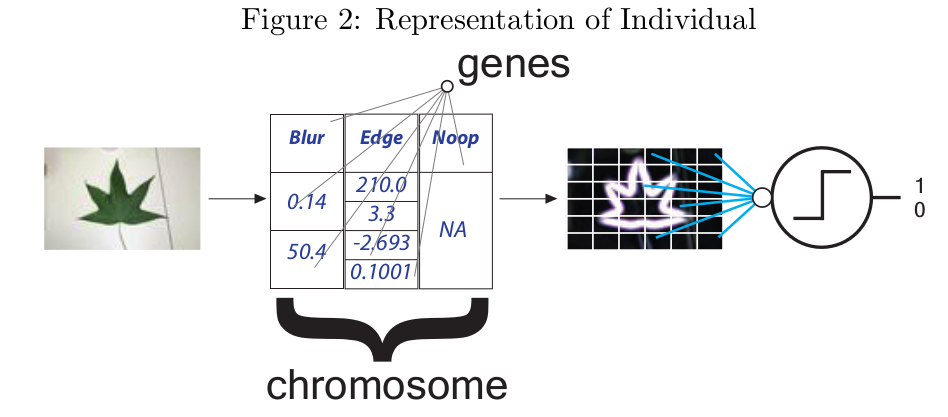
\includegraphics[width=0.8\textwidth]{helpful.png}
\caption{Most helpful figure}
\label{fig:helpful}
\end{figure}
\subsection{What was the most eye catching graphic displayed in the project report?}
See figure \ref{fig:catching}.
\begin{figure}[H]
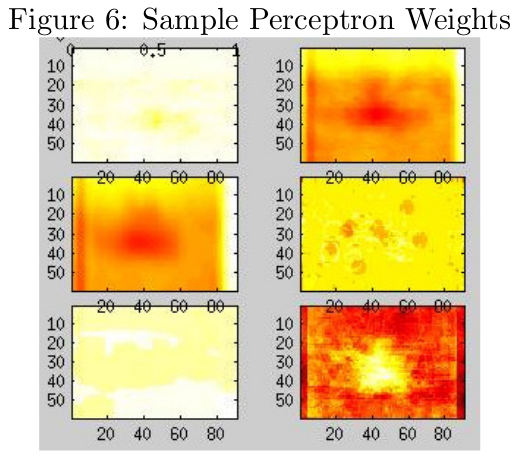
\includegraphics[width=0.8\textwidth]{catching.png}
\caption{Most catching figure}
\label{fig:catching}
\end{figure}
\subsection{Did you find it interesting? Why or why not?}
I haven't seen the combination of EA and Adaboost before, so it was interesting.

\section{Part III - What would you do differently}
\subsection{Would you accept the task (of improving the work done)?}
Yes
\subsection{What would you do differently?}
As the authors suggested the EA is not applied as it should have been. It evolves the weak classifiers which then get combined to form a strong one. The strong classifier should be included in the EA as well.
\subsection{Why do you expect better results?}
This approach would focus more on finding weak classifiers that are good in cooperating with other weak classifiers instead of just being evaluated on their own.
\subsection{How long would you estimate it would take you to improve upon the previous results?}
Full time and motivated? 2 weeks?
\subsection{How much of an improvement would you estimate you'd be able to achieve?}
The authors used a simple data set so the gain would probably be small on this data. On other data I don't know how this algorithm would perform, so I am not able to give an estimate.
\subsection{Visualization of data set}
No data set available.

\bibliographystyle{plain}
\bibliography{literature.bib}


\end{document}